%%%%%%%%%%%%%%%%%%%%%%%%%%%%%%%%%%%%%%%%%%%%%%%%%%%%%%%%%%%%%%%%%%%%%%
%%%%  NIGHT CHILDREN %%%%%%%%%%%%%%%%%%%%%%%%%%%%%%%%%%%%%%%%%%%%%%%%%%%%%%%
%%%%%%%%%%%%%%%%%%%%%%%%%%%%%%%%%%%%%%%%%%%%%%%%%%%%%%%%%%%%%%%%%%%%%%
\mysubsection{Night Child Virtues}{advancement-night-child-virtues}

\myemph{Unless otherwise specified, you can take each Virtue only once.}


  \mytable{Y Y Y} {
    \thead{Daredevil (Level 2+)} & \thead{Heroic (Level 4+)} & \thead{Legendary (Level 7+)} \\
  } {
    Freaky\Asterisk  & Bump\Asterisk  & Kismet III \\
    Kismet I & Bump Bump\Asterisk  &  Nuke\\
    More Freaky\Asterisk  &  Bump Bump Bump\Asterisk  &  Personality III \\
    More Pretty\Asterisk  & Bump Bump Bump Bump\Asterisk   &  Saves III \\
    More Stuff\Asterisk  & Kismet II & That One\Asterisk  \\
    Personality I & Personality II & - \\
    Pretty\Asterisk  & Saves II & -  \\
    Saves I & - & - \\
    Stuff\Asterisk   & - & - \\
}

\callout {
    \Asterisk This Virtue can be taken up to three times per \LVL.
}


\begin{multicols*}{2}

\myhighlight{Bump}{adv-night-child-bump}

Add or subtract 1 to a Looks, Weird, or Gear roll you just made.

\myhighlight{Bump Bump}{adv-night-child-bump-bump}

Add or subtract 2 to a Looks, Weird, or Gear roll you just made.

\myhighlight{Bump Bump Bump}{adv-night-child-bump-bump-bump}

Add or subtract 3 to a Looks, Weird, or Gear roll you just made.

\myhighlight{Bump Bump Bump Bump}{adv-night-child-bump-bump-bump-bump}

Add or subtract 4 to a Looks, Weird, or Gear roll you just made.


\myhighlight{Freaky}{adv-night-child-freaky}

Roll your Weird die and apply the result to your Adventurer.

\cbreak

\myhighlight{Kismet I-III}{adv-night-child-kismet}

Advance \mybold{all} aspects of your \mybold{Kismet} - \DEATH, \INJURY, and \INSANITY - to the next named level.


\myhighlight{More Freaky}{adv-night-child-more-freaky}

Raise you Weird die \DCUP.

\myhighlight{More Pretty}{adv-night-child-more-pretty}

Raise you Looks die \DCUP.

\myhighlight{More Stuff}{adv-night-child-more-stuff}

Raise you Gear die \DCUP.

\end{multicols*}
\newpage

\begin{center}
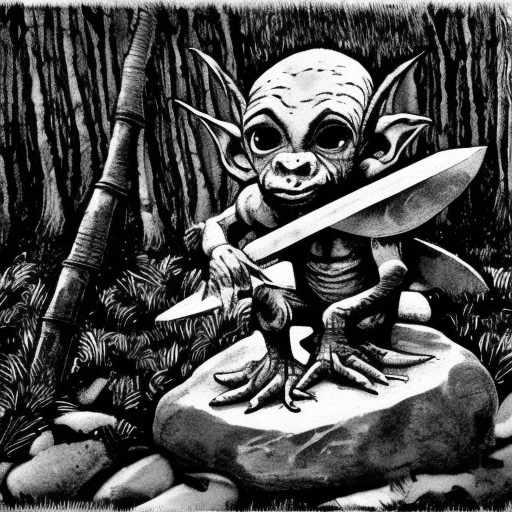
\includegraphics{advancement/NightChild}
\end{center}

\begin{multicols*}{2}

\myhighlight{Nuke}{adv-night-child-nuke}

At any time, you may open yourself to the Void, channeling it through your body. Roll your Looks, Weird, and Gear dice and deal \SUM x2 damage to all Monsters Close or Nearby (Save for half damage). After you roll the damage, immediately roll on the \mypg{Ruin}{table-ruin} table.

\myhighlight{Personality I-III}{adv-night-child-personality}

Advance two \mybold{different} aspects of your \mybold{Personality} \DCUP. 


\myhighlight{Pretty}{adv-night-child-pretty}

Roll your Looks die and apply the result to your Adventurer.

\cbreak

\myhighlight{Saves I-III}{adv-night-child-saves}

Advance \mybold{all} Saves to the next named level (Defenseless to Preserved; Preserved to Protected; etc). 

\myhighlight{Stuff}{adv-night-child-stuff}

Roll your Gear die and apply the result to your Adventurer.

\myhighlight{That One}{adv-night-child-that-one}

Choose a Looks, Weird, or Gear result as if you rolled the appropriate die.  For example, if your Gear die is a d8, you can choose any Gear result from 1 to 8.

\end{multicols*}
